\chapter{Case Study 2: Another good chapter}
\section{Section1}
\section{Section2}

\begin{figure}[t]
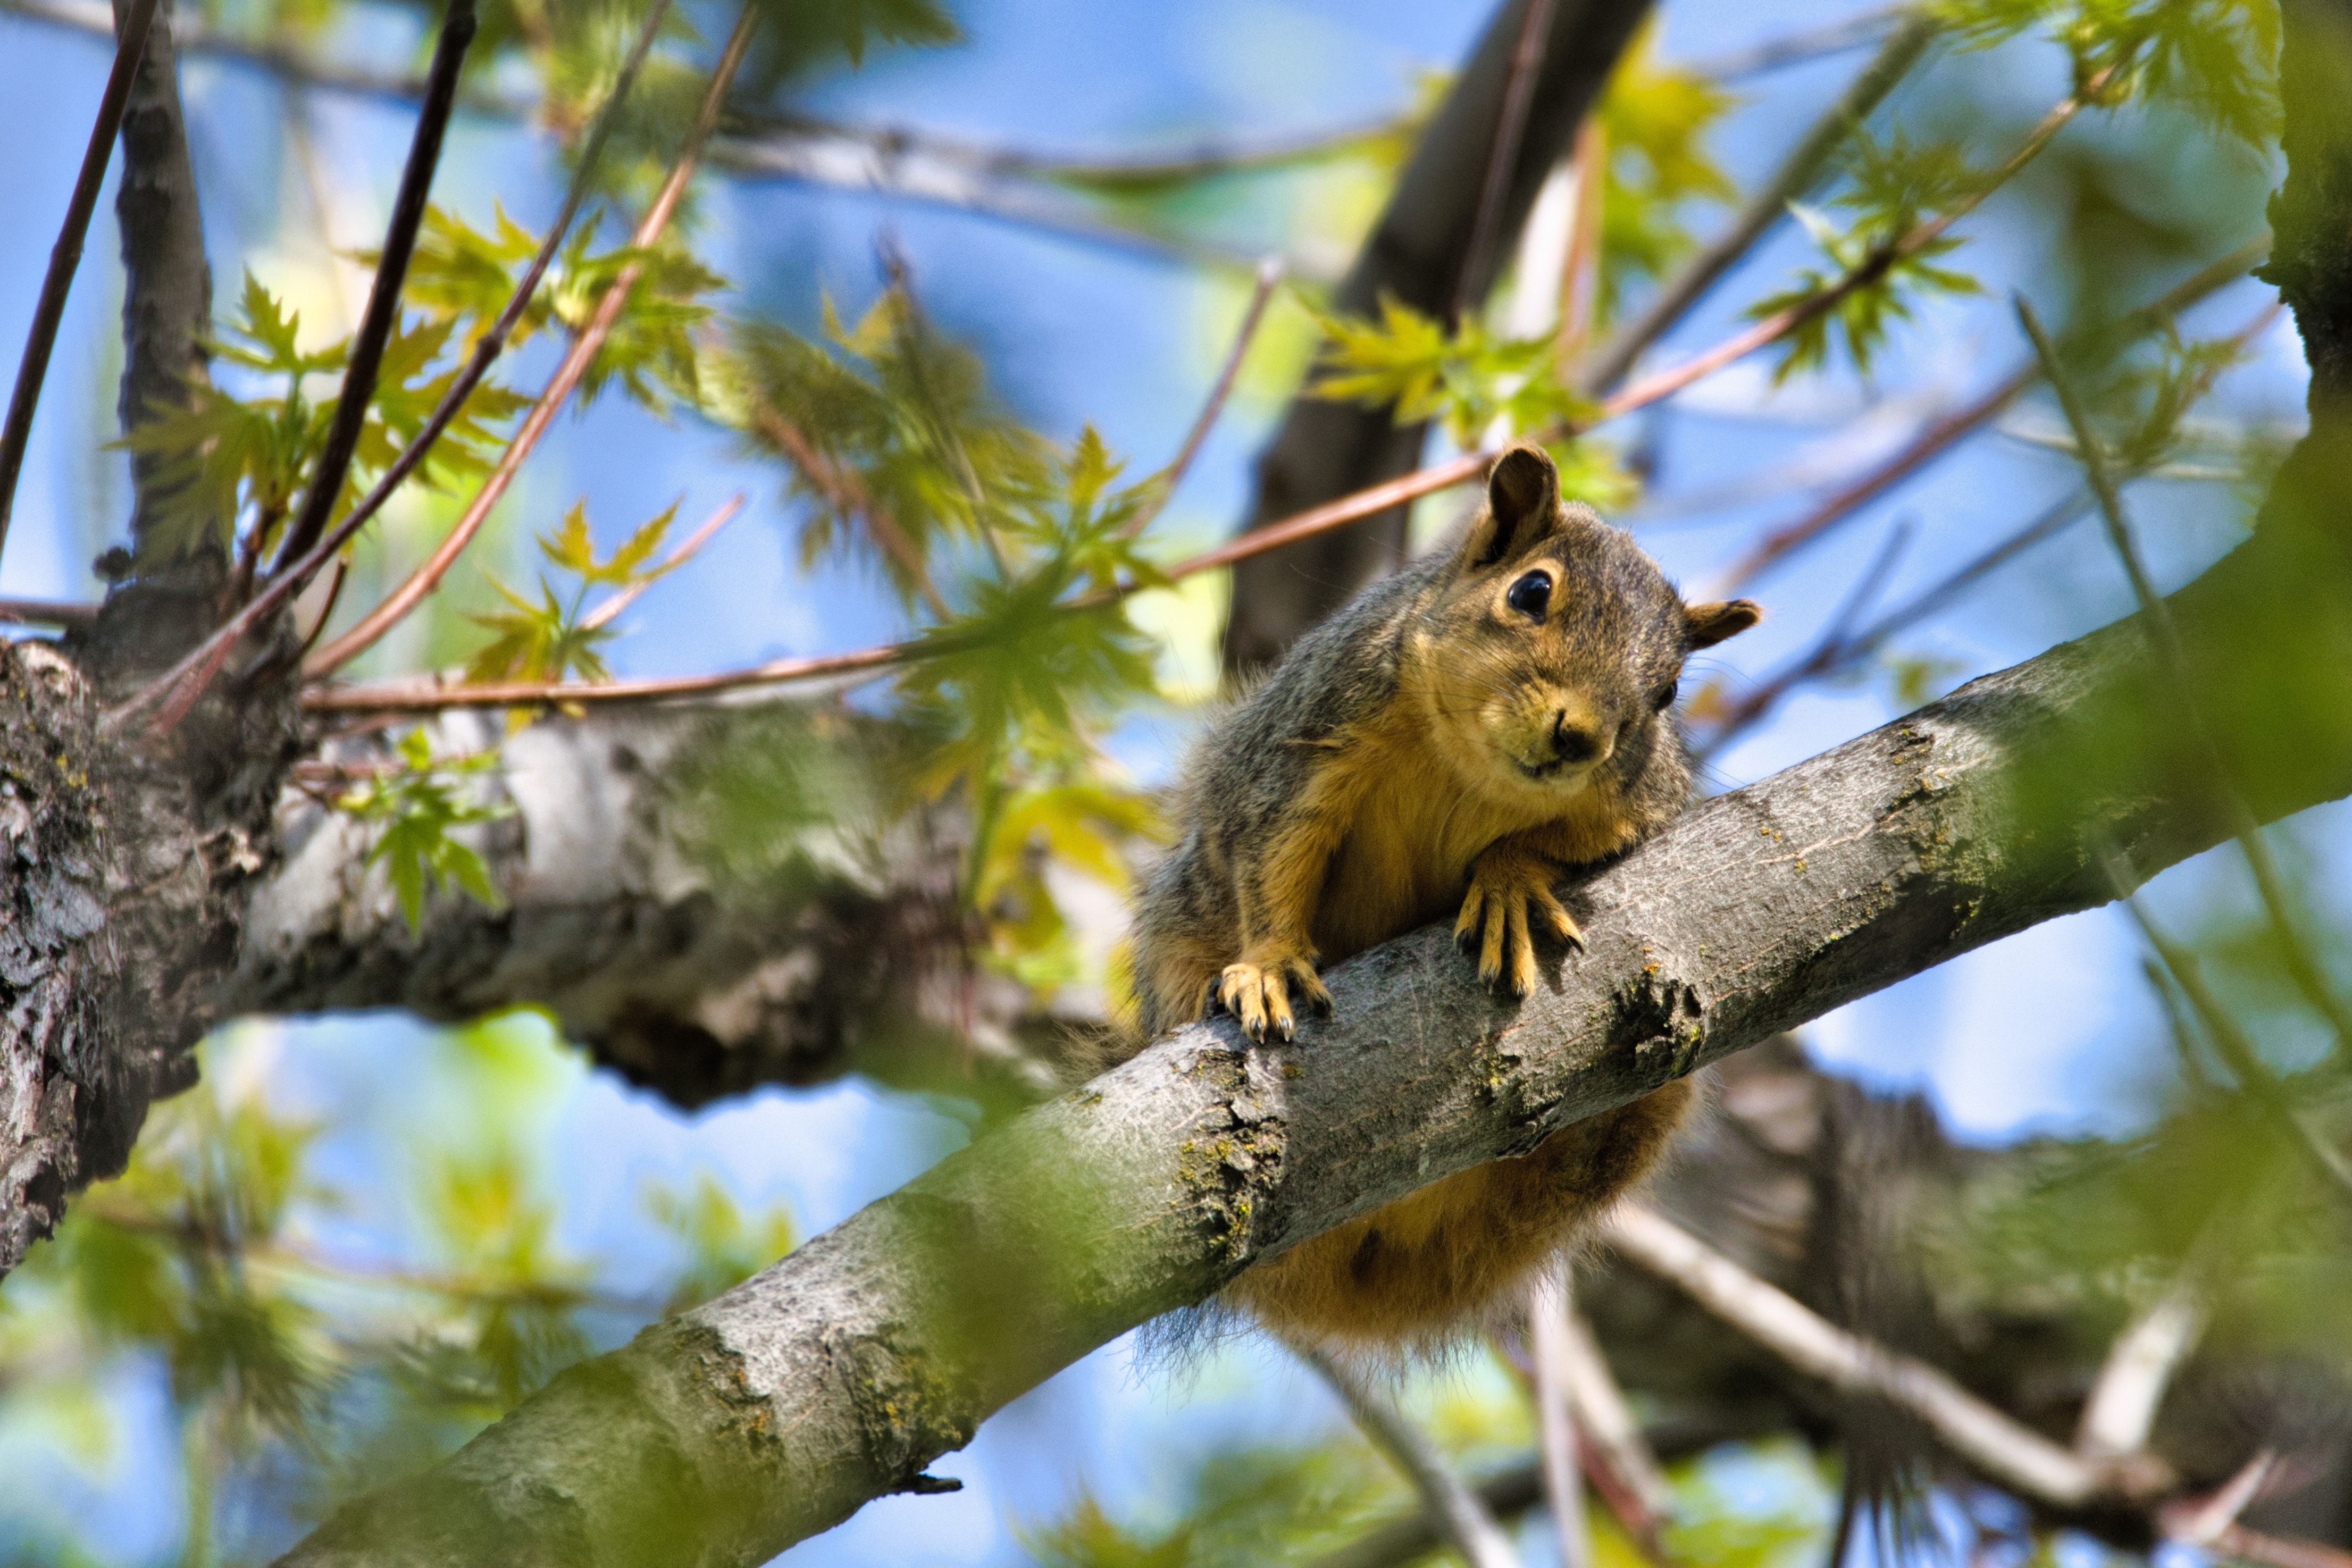
\includegraphics[width=8cm]{demo.jpg}
\centering
  \caption{A very good friend, with good news.}
    \label{fig:demo}
\end{figure}
he other side, if you are only interested on
certain va for documents that include \gls{maths}.lues you can use the contour plot, you 
can use the contour plot, you can use the contour 
plot, you can use the contour plot, you can use 
the contour plot, you \acrshort{vgd} can use the contour plot, 
you can use the contour.  The table \ref{table:1} is an example of referenced \LaTeX elements.
 
\begin{table}[h!]
\centering
\begin{tabular}{||c c c c||} 
 \hline
 Col1 & Col2 & Col2 & Col3 \\ [0.5ex] 
 \hline\hline
 1 & 6 & 87837 & 787 \\ 
 2 & 7 & 78 & 5415 \\
 3 & 545 & 778 & 7507 \\
 4 & 545 & 18744 & 7560 \\
 5 & 88 & 788 & 6344 \\ [1ex] 
 \hline
\end{tabular}
\caption{Table to demonstrate captions and labels}
\label{table:1}
\end{table}

%% Just to fill out the table of contents
\chapter{Case Study 3: Brilliant!}
\section{Section1}
\section{Section2}